\chapter{Checklists}
\label{ch:checklists}

\section{Pre-Flight Checklist}\label{cl:preflight}
 The following pre-flight procedures will be completed before every flight. 
    \subsection{Payload} 
        \subsubsection{} Fill payload box with MEDLOG. Ensure in-flight shifting will be minimized by packing the box tightly. Use newspaper or foam to fill in gaps and prevent sliding.
        \subsubsection{} Weigh payload box to ensure it weighs no more than 5lb. 
        \subsubsection{} Place the payload box into the Tyvek bag, place into the payload compartment, close the door, and lock with the attached padlock. Remember the code and ensure the personnel receiving the drone also know the code.

    \subsection{Battery} 
        \subsubsection{} Ensure you have two fully charged 6C 22.2V 23 Ah LiPo Batteries. Save one as a back up. Check the battery voltage. If using a 22.2V battery, the voltage should be 25.2V across all cells when fully charged. 
        \subsubsection{} Navigate to Full Parameter List and verify the following parameters:
        \begin{itemize}
            \item BATT\_ARM\_MAH = 5750 (or 25\% maximum battery capacity)
            \item BATT\_ARM\_VOLT = 22
            \item BATT\_CAPACITY = 23000 (verify with your actual battery)
            \item BATT\_MONITOR = 4
        \end{itemize}
        

    \subsection{Drone Set Up} 
        \subsubsection{} Place MARS on a safe, level takeoff location. This takeoff location must correspond with the takeoff location marked on the mission plan.
        \subsubsection{} Secure battery into the designated compartment on MARS. Secure with Velcro strap (primary) or duct tape (alternate). Plug in the battery and ensure components are receiving power. 
        \subsubsection{} Inspect the drone for the following:
        \begin{itemize}
            \item propellers are oriented in the correct directions (the direction of spin should be opposing between all adjacent propellers)
            \item payload is securely attached with padlock locked. 
            \item Verify that green and red signal lights are on and visible. 
        \end{itemize}
        \subsubsection{} Give thumbs up to the GCS operator when inspection is complete and no issues are found. Clear the takeoff point of all personnel and equipment in a 5m radius to ensure a safe takeoff. If at any point drone maintenance is required on the takeoff point, notify all ground control personnel and ensure the drone is not armed. 
        \subsubsection{} Call the catcher at the landing site to confirm the following: 
        \begin{itemize}
            \item They are at the landing site, awaiting receipt of the drone. 
            \item They have an estimated time of arrival for MARS. 
            \item They know the padlock combination. 
            \item You may not launch MARS without the catcher’s approval. 
        \end{itemize}
    
    \subsection{Ground Control Station (GCS)} 
        \subsubsection{} Using an external computer or laptop
            \paragraph{} Power on the ground control computer and connect to the \ac{gcs} radio using an Ethernet cable. 
            \paragraph{} Configure the \ac{gcs} computer’s ethernet adapter settings as follows:
            \begin{itemize}
                \item Static IP address: 10.223.148.10
                \item Subnet Mask: 255.255.0.0
                \item Ping \ac{kach} \ac{gcs} radio IP address (default is 10.223.148.158) to verify that packets are sent and received between the computer and the radio.
                \begin{figure}
                    \centering
                    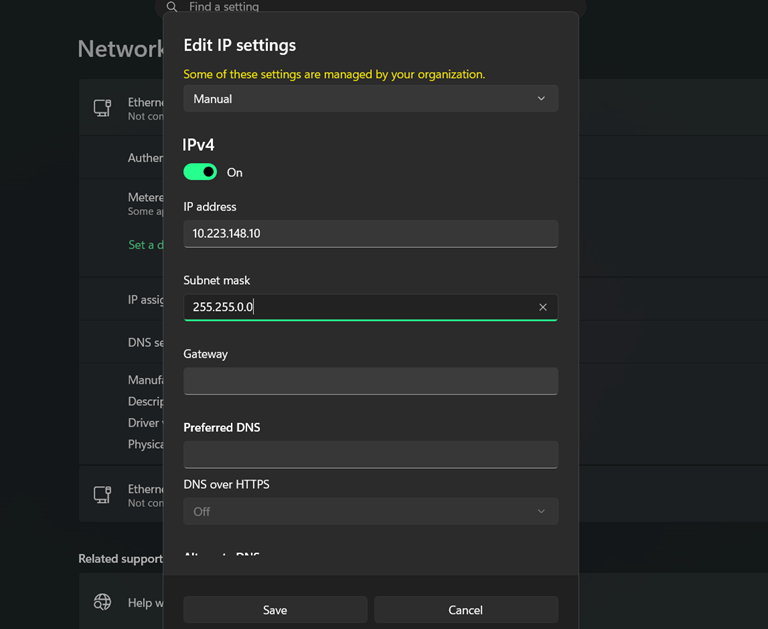
\includegraphics[width=0.5\linewidth]{IP_settings}
                    \caption{Manual Wifi Interface Settings}
                    \label{fig:placeholder}
                \end{figure}
            \end{itemize}
        \subsubsection{} Connecting to the built-in \ac{gcs} computer over the internet or SSH.

    \subsection{GCS Software} 
        \subsubsection{Mission Planner (Primary)} 
            \paragraph{} Open Mission Planner on the GCS computer. Use version 1.3.83 or newer.
            \paragraph{} In the top right corner of the application, select UDP in the connection protocol dropdown menu. To the immediate right, select a baud rate of 57600.
            \paragraph{} Click “Connect” and enter a local port number of 14560. If the drone is already powered on, the software should connect to the drone’s flight controller after a few seconds and mission planner will load the drone’s saved parameters.
        \subsubsection{QGroundControl (QGC - Alternate)} QGC should automatically receive the UDP stream from the drone radio on port 14560 and connect upon launching the app. 

    \subsection{Load Mission Plan} 
        \subsubsection{} Load the mission plan from a saved file. In Mission Planner, go to Plan $\rightarrow$ Load File. Alternatively, plan a new one in the Plan tab. (Not recommended for routine flights).
        \subsubsection{} Verify that the mission looks correct. Double check the following mission settings on the left of the screen: 
        \begin{itemize}
            \item Initial waypoint altitude 
            \item Hover speed 
            \item Launch altitude 
        \end{itemize}
        \subsubsection{} Upload mission plan to MARS by clicking ``Write” in Misson Planner or ``Upload” in QGC.

    \subsection{Failsafe Configuration} Navigate to the Full Parameter List and verify the following settings:
        \subsubsection{Battery} 
        \begin{itemize}
            \item BATT\_CRT\_MAH = 2300 (Or 10\% of maximum battery capacity)
            \item BATT\_CRT\_VOLT = 20
            \item BATT\_FS\_CRT\_ACT = 1
            \item BATT\_FS\_LOW\_ACT = 2
            \item BATT\_LOW\_MAH = 3450
            \item BATT\_LOW\_TIMER = 10
            \item BATT\_LOW\_VOLT = 21
        \end{itemize}
        \subsubsection{Geofence} 
        \begin{itemize}
            \item FENCE\_ENABLE = 1
            \item FENCE\_ACTION = 1
            \item FENCE\_ALT\_MAX = 200
            \item FENCE\_ALT\_MIN = -200
            \item FENCE\_AUTOENABLE = 0
            \item FENCE\_OPTIONS = 0
            \item FENCE\_TYPE = 5
        \end{itemize}
        \subsubsection{RTL} 
        \begin{itemize}
            \item RTL\_ALT = 1000
            \item RTL\_ALT\_FINAL  = 0
            \item RTL\_ALT\_TYPE = 0
            \item RTL\_CLIMB\_MIN = 0
            \item RTL\_CONE\_SLOPE = 3
            \item RTL\_LOIT\_TIME = 5000
            \item RTL\_OPTIONS = 0
            \item RTL\_SPEED = 0

        \end{itemize}
        \subsubsection{Miscellaneous} 
        \begin{itemize}
            \item FS\_GCS\_TIMEOUT = 5
            \item FS\_OPTIONS = 16
            \item FS\_THR\_ENABLE = 1
            \item FS\_VIBE\_ENABLE = 1
        \end{itemize}
        \subsubsection{Arming Checks} 
        \begin{itemize}
            \item ARMING\_MIS\_ITEMS = 73 (takeoff, land, RTL required to arm)
            \item ARM\_NEED\_LOC = 1
        \end{itemize}
            
\section{Post-Flight Checklist}\label{cl:postflight}

\section{Emergency Procedures Checklist}\label{cl:emergencyprocedures}

